\section{Unsupervised Learning}
The classical clustering problem starts with a set of $n$ objects and an $n \times n$ matrix $A$ of pairwise similarities that gives us an edge-weighted graph $G$. The goal of the clustering problem is to partition the vertices of $G$ into maximally homogeneous groups (clusters). Usually the graph $G$ is an undirected graph.
\image{img/clustering}{The "classical" clustering problem.}{0.8}

\subsection{K-means}
K-means is an iterative clustering algorithm that follows these steps:
\begin{itemize}
	\item \textbf{Initialize:} pick $K$ random points as cluster centers.
	\image{img/kmeans1}{Initialization with $K=2$.}{0.24}
	\item \textbf{Alternate:}
	\begin{enumerate}
		\item assign data points to closest cluster center.
		\item change the cluster center to the average of its assigned points.
		\begin{figure}[H]
			\begin{minipage}[t]{0.42\linewidth} 
				\centering
				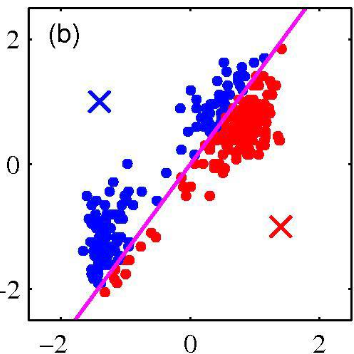
\includegraphics[width=0.58\textwidth]{img/kmeans2}
				\caption{Iterative step 1.}
			\end{minipage}        
			\hspace{2.5cm}
			\begin{minipage}[t]{0.42\linewidth} 
				\centering
				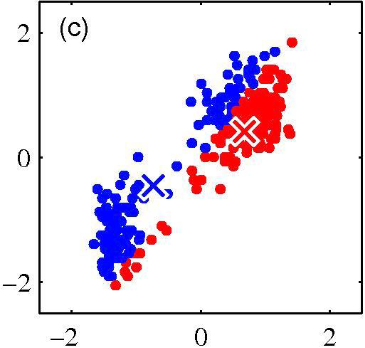
\includegraphics[width=0.58\textwidth]{img/kmeans3}
				\caption{Iterative step 2.}
			\end{minipage}
		\end{figure}
		\FloatBarrier
	\end{enumerate}
	\item \textbf{Stop:} when no points' assignments change.
	\begin{figure}[H]
		\begin{minipage}[t]{0.42\linewidth} 
			\centering
			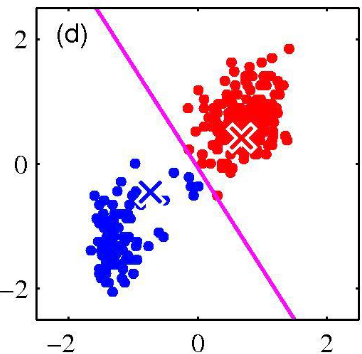
\includegraphics[width=0.58\textwidth]{img/kmeans4}
			\caption{Repeat until convergence.}
		\end{minipage}        
		\hspace{2.5cm}
		\begin{minipage}[t]{0.42\linewidth} 
			\centering
			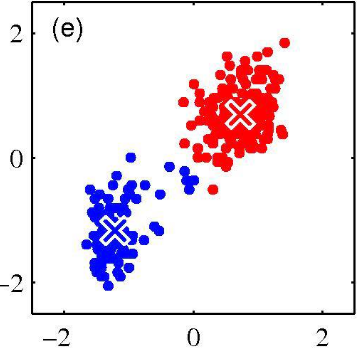
\includegraphics[width=0.58\textwidth]{img/kmeans5}
			\caption{Final output.}
		\end{minipage}
	\end{figure}
\end{itemize}
\paragraph*{Properties of K-means.} K-means has the following properties:
\begin{itemize}
	\item It is guaranteed to converge in a finite number of steps.
	\item It minimizes an objective function (compactness of clusters):
	$$\sum_{i \in \text{clusters}} \Biggl\{ \sum_{j \in \text{elements of i-th cluster}} ||x_j - \mu_i||^2 \Biggr\}$$
	where $\mu_i$ is the center of cluster $i$.
	\item It assigns data points to closest cluster center in $O(Kn)$ and it changes the cluster center to the average of its points in $O(n)$.
\end{itemize}
It is possible to say that K-means is a very simple and efficient method but, on the other hand, it converges to a local minimum of the error function and it needs to pick $K$ initial points, hence proving to be very sensitive to the initialization step.

\subsection{Images as graphs}
It is also possible to consider images as graphs, which can be described in the following way:
\begin{itemize}
	\item A node for every pixel.
	\item An edge between every pair of pixels (or every pair of "sufficiently close" pixels).
	\item Each edge is weighted according to the affinity or similarity of the two nodes.
\end{itemize}  
\image{img/imageasgraph}{Image as a graph.}{0.7}
If we suppose to represent each pixel with a feature vector $x$ and to define a distance function appropriate for this feature representation, then we can convert the distance between two feature vectors into an \textbf{affinity} with the help of a Guassian kernel:
$$exp\left(-\frac{1}{2\sigma^2} dist(x_i, x_j)^2\right)$$
The scale affects the affinity:
\begin{itemize}
	\item Small $\sigma$: group only nearby points.
	\item Large $\sigma$: group distant points.
\end{itemize}

\subsection{Eigenvector-based clustering}
Let us represent a cluster using a vector $x$ whose $k$-th entry captures the participation of node $k$ in that cluster. If a node does not participate in a cluster, the corresponding entry is zero.\\
We also impose the restriction that $x^Tx = 1$ in order to avoid the trivial solution $x=0$.\\
We want to maximize:
$$\sum_{i=1}^n \sum_{j=1}^n w_{ij} x_i x_j = x^TAx$$
which measures the cluster's cohesiveness.\\
This is an \textbf{eigenvalue problem}, which consists in choosing the eigenvector of $A$ corresponding to the largest eigenvalue.\\
We have that $A$ is a square affinity matrix $n \times n$, where $n$ is the number of nodes. Two important theorems hold:
\begin{enumerate}
	\item if $A = A^T$, then $A$ is symmetric and $A$ only has "\textit{real}" eigenvalues.
	\item if $A$ is symmetric, then $x^TAx$ is the largest eigenvalue. 
\end{enumerate}
For each node $i$, $x_i$ represents the measure of centrality to the cluster and it is defined as:
$$x_i = \begin{cases}
\neq 0 \text{  if } i \in C\\
= 0 \text{  if } i \notin C
\end{cases}$$
From the following image we can see that it could be possible to find clusters by visual inspection of the eigenvectors.

\begin{figure}[H]
	\begin{minipage}[t]{0.49\linewidth} 
		\centering
		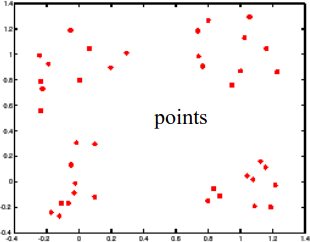
\includegraphics[width=1\textwidth]{img/eigenpoints}
	\end{minipage}        
	\hspace{1cm}
	\begin{minipage}[t]{0.49\linewidth} 
		\centering
		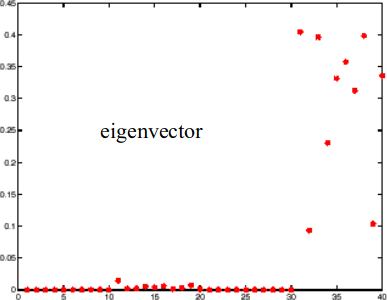
\includegraphics[width=1\textwidth]{img/eigenvectors}
	\end{minipage}
\end{figure}
In case we must extract more than two clusters from the eigenvectors, we can recursively split each side to get a tree, continuing till the eigenvalues are too small. 
\paragraph*{Clustering by eigenvectors: Algorithm.} The algorithm that builds the clusters through the eigenvectors is composed by the following steps:
\begin{enumerate}
	\item Construct (or take as input) the affinity matrix $A$
	\item Compute the eigenvalues and eigenvectors of $A$
	\item Repeat
	\item $\quad$ Take the eigenvector corresponding to the largest unprocessed eigenvalue.
	\item $\quad$ Zero all the components corresponding to elements that have already been clustered
	\item $\quad$ Threshold the remaining components to determine which elements belong to this cluster
	\item $\quad$ If all elements have been accounted for, there are sufficient clusters 
	\item Until there are sufficient clusters
\end{enumerate}

\subsubsection{Clustering as graph partitioning}
Let $G=(V,E,w)$ be an undirected weighted graph (affinity matrix is symmetric). Given a \textit{cut} $(A,B)$, with $B=V \backslash A$, define:
$$cut(A,B) = \sum_{i \in A} \sum_{j \in B} w(i,j)$$
\image{img/minCut}{Minimum cut problem.}{0.8}
In the MinCut problem, the sum of the weights of the edges which cross the cut should be as small as possible.\\
The MinCut clustering is advantageous because is solvable in polynomial time but, on the other hand, it favors highly unbalanced clusters (often with isolated vertices), indeed, it only measures what happens between the clusters and not what happens within the clusters.
\image{img/minCut2}{Minimum cut disadvantage.}{0.45}

\subsubsection{Normalized Cut}
In order to overcome the problem of unbalanced clusters, \textbf{Normalized Cut} is used and it is defined by:
$$Ncut(A,B) = \underbrace{cut(A,B)}_{\text{Between A and B}}\left( \underbrace{\frac{1}{vol(A)} + \frac{1}{vol(B)}}_{\text{Within A and B}}\right)$$
where $vol(A)$ is the volume of the set $A$ given by $vol(A) = \sum_{i \in A}d_i,~A \subseteq V$ and $d_i = \sum_j w_{i,j}$ is the degree of nodes (sum of weights).\\
Normalized cut has the advantage of taking into consideration what happens within the clusters by considering $vol(A)$ and $vol(B)$.
\begin{figure}[H]
	\begin{minipage}[t]{0.46\linewidth} 
		\centering
		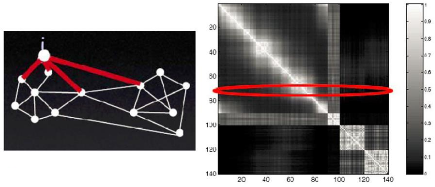
\includegraphics[width=0.9\textwidth]{img/degreeNodes}
		\caption{Degree of nodes.}
	\end{minipage}        
	\hspace{1cm}
	\begin{minipage}[t]{0.49\linewidth} 
		\centering
		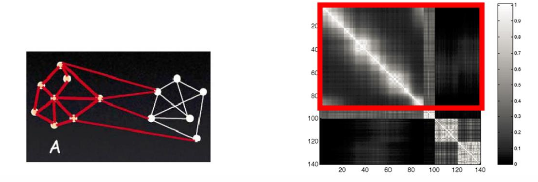
\includegraphics[width=1\textwidth]{img/volumeSet}
		\caption{Volume of a set.}
	\end{minipage}
\end{figure}

\subsubsection{Graph Laplacians}
The main tools for spectral clustering are graph Laplacian matrices, there exists a whole field dedicated to the study of those matrices, called spectral graph theory.  In this section we want to define different graph Laplacians and point out their most important properties.

\paragraph{The unnormalized graph Laplacian.} The  \textbf{unnormalized graph Laplacian} matrix is defined as:
$$L = D - W$$
where:
\begin{itemize}
	\item $D$ is a diagonal matrix whose main diagonal is made of the degrees of the nodes in the graph.
	\item $W$ is the affinity matrix, in which the diagonal elements are all $0s$ by definition. If the graph is unweighted (as per the following example), $W$ only contains $1s$ (adjacent nodes) and $0s$ (non-adjacent nodes).
\end{itemize}
This is an example of the degree matrix $D$ and the affinity matrix $W$ in relation to the graph of the next page.
\begin{figure}[H]
	\begin{minipage}[t]{0.49\linewidth} 
		\centering
		$$ D = \begin{bmatrix}
		2 & 0 & 0 & 0 & 0 & 0 \\
		0 & 4 & 0 & 0 & 0 & 0 \\
		0 & 0 & 4 & 0 & 0 & 0 \\
		0 & 0 & 0 & 1 & 0 & 0 \\
		0 & 0 & 0 & 0 & 3 & 0 \\
		0 & 0 & 0 & 0 & 0 & 2 \\
		\end{bmatrix}$$
		\caption{Degree matrix $D$.}
	\end{minipage}        
	\hspace{1cm}
	\begin{minipage}[t]{0.49\linewidth} 
		\centering
		$$ W = \begin{bmatrix}
		0 & 1 & 1 & 0 & 0 & 0 \\
		1 & 0 & 1 & 1 & 1 & 0 \\
		1 & 1 & 0 & 0 & 1 & 1 \\
		0 & 1 & 0 & 0 & 0 & 0 \\
		0 & 1 & 1 & 0 & 0 & 1 \\
		0 & 0 & 1 & 0 & 1 & 0 \\
		\end{bmatrix}$$
		\caption{Affinity matrix $W$.}
	\end{minipage}
\end{figure}

The elements of $L$ are given by:
$$
L _ { i , j } = \left\{ \begin{array} { l l } { \operatorname { d } \left( v _ { i } \right) } & { \text { if } i = j } \\ 
{ - 1 } & { \text { if } i \neq j \text { and } v _ { i } \text { is adjacent to } v _ { j } } \\ 
{ 0 } & { \text { otherwise } } \end{array} \right.
$$
where $d(v_i)$ is the degree of the vertex $i$.
\image{img/graphLaplacian}{Example of laplacian graph.}{0.85}

The matrix $L$ satisfies the following properties:
\begin{enumerate}
	\item For all vectors $f$ in $\mathbb{R}^n$, we have:
	$$f ^ { \top } L f = \frac { 1 } { 2 } \sum _ { i, j = 1 } ^ { n } w _ { i j } \left( f _ { i } - f _ { j } \right) ^ { 2 }$$
	This is proved by the definition of $d_i$:
	$$\begin{aligned} 
	f ^ { \top } L f & = f ^ { \top } D f - f ^ { \top } W f = \sum _ { i=1 }^n d _ { i } f _ { i } ^ { 2 } - \sum _ { i , j =1 }^n f _ { i } f _ { j } w _ { i j } \\ 
	& = \frac { 1 } { 2 } \left( \sum _ { i=1 }^n \left( \sum _ { j=1 }^n w _ { i j } \right) f _ { i } ^ { 2 } - 2 \sum _ { i, j=1 }^n f _ { i } f _ { j } w _ { i j } + \sum _ { j=1 }^n \left( \sum _ { i=1 }^n w _ { i j } \right) f _ { j } ^ { 2 } \right) \\ 
	& = \frac { 1 } { 2 } \sum _ { i ,j=1 }^n w _ { i j } \left( f _ { i } - f _ { j } \right) ^ { 2 } 
	\end{aligned}$$
	 
	\item $L$ is symmetric (by assumption) and positive semi-definite. The symmetry of $L$ follows directly from the symmetry of $W$ and $D$. The positive semi-definiteness is a direct consequence of the first property, which shows that 	$f ^ { T } L f \geq 0$
	 
	\item The smallest eigenvalue of $L$ is 0, the corresponding eigenvector is the constant 1 vector.
	\item $L$ has $n$ non-negative, real-valued eigenvalues $0 = \lambda _ { 1 } \leq \lambda _ { 2 } \leq \ldots \leq \lambda _ { n }$
\end{enumerate}

First relation between spectrum and clusters:
\begin{itemize}
	\item Multiplicity of eigenvalue $\lambda_1=0$ is the number of connected components $A_1, \dots, A_k$ of the graph. Note that the multiplicity of an eigenvalue is defined as the number of eigenvectors associated with that specific eigenvalue.
	\item The eigenspace is spanned by the characteristic function of these components, meaning that the members of a cluster share the same value ($1$) for a certain characteristic function. This is the same as stating that those eigenvectors are piecewise constant, since if we apply the characteristic function to all of them, we always get the same value.
\end{itemize}

\begin{figure}[H]
	\begin{minipage}[t]{0.49\linewidth} 
		\centering
		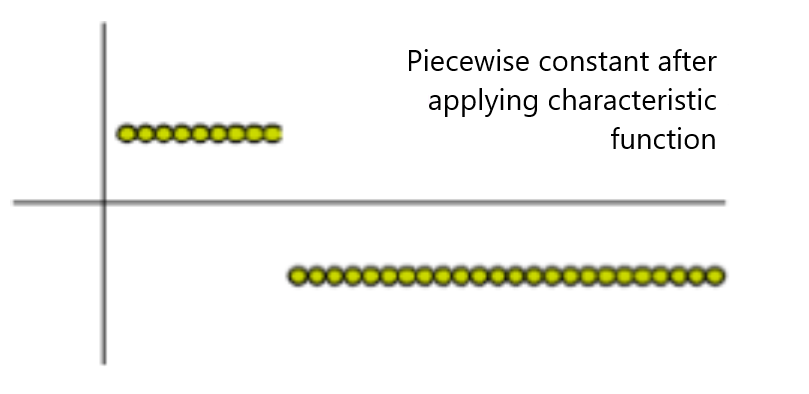
\includegraphics[width=1\textwidth]{img/idealSolutionClustering}
		\caption{Eigenvectors in the new space: finding the clusters is easier}
	\end{minipage}        
	\hspace{1cm}
	\begin{minipage}[t]{0.49\linewidth} 
		\centering
		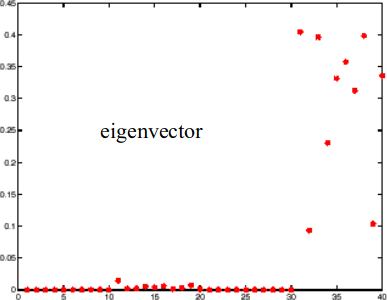
\includegraphics[width=1\textwidth]{img/eigenvectors}
		\caption{Original representation of the eigenvectors}
	\end{minipage}
\end{figure}


\paragraph{The normalized graph Laplacians.} There are two matrices which are called normalized graph Laplacians in the literature. Both matrices are closely related to each other and are defined as:
$$\begin{array} { l } { L _ { \mathrm { sym } } = D ^ { - 1 / 2 } L D ^ { - 1 / 2 } = I - D ^ { - 1 / 2 } W D ^ { - 1 / 2 } } \\ { L _ { \mathrm { rw } } = D ^ { - 1 } L = I - D ^ { - 1 } W } \end{array}$$
We denote the first matrix by $L_{sym}$ as it is a symmetric matrix, and the second one by $L_{rw}$ as it is closely connected to a random walk.
 
\subsubsection{Solving Ncut} 
Any cut $(A,B)$ can be represented by a binary indicator vector $x$:
$$x_i = \begin{cases}
+1 \text{  if } i \in A\\
-1 \text{  if } i \in B
\end{cases}$$
It can be shown that:
$$min_x ~ Ncut(x) = min_y \underbrace{\frac{y'(D-W)y}{y'Dy}}_{\text{Rayleigh quotient}}$$
subject to the constraint that $y ^ { \prime } D1 = \sum_{i} y_{i} d _ { i } = 0$ (with $y _ { i } \in \{ 1 , - b \}$ (relaxation introducing also real values). Indeed, $y$ is an indicator vector with 1 in the $i$-th position if the $i$-th feature point belongs to $A$, negative constant ($-b$) otherwise ). This is \textbf{NP-Hard}!\\
The huge Ncut time complexity brings us to take into consideration an approximation of it. If we relax the constraint that $y$ be a discrete-valued vector and allow it to take on real values, the original problem
$$\min _ { y } \frac { y ^ { \prime } ( D - W ) y } { y ^ { \prime } D y }$$
will be equivalent to:
$$\min _ { y } y ^ { \prime } ( D - W ) y \quad \text { subject to } y ^ { \prime } D y = 1$$
This amounts to solve a \textit{generalized} eigenvalue problem:
$$\underbrace{(D-W)}_{Laplacian}y=\lambda D y$$
It is possible then, to sum up the different steps of the Normalized Cut algorithm as:
\begin{enumerate}
	\item Represent the image as a weighted graph $G = (V,E)$, compute weight of each edge and summarize in $D$ and $W$.
	\item Solve $(D-W)y = \lambda Dy$ for the eigenvector with the second smallest eigenvalue.
	\item Use the entries of the eigenvector to bipartition the graph.
\end{enumerate}
We started from an NP-Hard problem and through relaxation we reached a feasible solution. However, we have not the guaranteed that the relaxed solution is in one to one correspondence.

\paragraph*{The effect of relaxation.} Through relaxation we lose some precision in the final solution. 
Note that the original Ncut problem returns binary values $(-1,1)$, indicating clustering membership. The relaxed version, on the right, returns continuous values. It may happen that some points do not clearly belong to a specific cluster, as they are close to the margin between the two clusters. For this reason the relaxed solution is not always in a one-to-one correspondence with the original problem, and choosing a ``correct'' threshold is very important.
\imageb{img/relaxation1}{0.8}

\subsubsection{Random walk interpretation} 
The Ncut problem can be also formalized in terms of random walk, since we want to find a cut that reduces the probability of jumping between nodes of different clusters. The problem can be defined as building a Markov chain where each data point is a state, connected to all other states with some probability. With our affinity $W$ and degree $D$, the stochastic matrix is:
$$P=D^{-1}W$$
which is the row-normalized version of $W$, so each entry $P(i,j)$ is a probability of "\textit{walking}" to state $j$ from state $i$.
\imageb{img/randomWalk}{0.20}
Probability of a walk through states $( s _ { 1 } , \dots , s _ { m })$ is given by:
$$P \left( s _ { 1 } , \ldots , s _ { 2 } \right) = P \left( s _ { 1 } \right) \prod _ { i = 2 } ^ { m } P \left( s _ { i } , s _ { i - 1 } \right)$$
Suppose we divide the states into two groups, and minimize the probability of jumping between the two groups. Formulate this as an eigenvector problem:
$$P y = \lambda y$$
where the component of vector $y$ will give the segmentation.\\
We can also precise that:
\begin{itemize}
	\item $P$ is a stochastic matrix.
	\item The largest eigenvalue is 1, and its eigenvector is the all-one vector 1. Not very informative about segmentation.
	\item The second largest eigenvector is orthogonal to the first, and its components indicate the strongly connected sets of states.
	\item Meila and Shi (2001) showed that minimizing the probability of jumping between two groups in the Markov chain is equivalent to minimizing Ncut.
\end{itemize}
\begin{thm}[Random Walk Proposition] $(\lambda, y)$ is a solution to $Py = \lambda y$ if and only if:
	\begin{itemize}
		\item $1-\lambda$ is an eigenvalue of $(D-W)y = \lambda D y$
		\item $y$ is an eigenvector of $(D-W)y = \lambda Dy$
	\end{itemize} 
	\textbf{Proof:}
	$$\begin{array} { l l } { P y = \lambda y } & { \Leftrightarrow \quad - P y = - \lambda y } \\
	 { } & { \Leftrightarrow \quad y - P y = y - \lambda y } \\
	 { } & { \Leftrightarrow \quad ( I - P ) y = ( 1 - \lambda ) I y } \\
	 { } & { \Leftrightarrow \quad \left( D ^ { - 1 } D - D ^ { - 1 } W \right) y = ( 1 - \lambda ) D ^ { - 1 } D y } \\
	 { } & { \Leftrightarrow \quad D ^ { - 1 } ( D - W ) y = D ^ { - 1 } ( 1 - \lambda ) D y } \\
	 { } & { \Leftrightarrow \quad ( D - W ) y = ( 1 - \lambda ) D y } \end{array}$$
\end{thm}
The problem is to find a cut $(A,B)$ in a graph $G$ such that a random walk does not have many opportunities to jump between the two clusters.\\
This is equivalent to the Ncut problem due to the following relation:
$$Ncut(A,B) = P(A|B) + P(B|A)$$
\subsubsection{2-way Ncut}
\begin{enumerate}
	\item Compute the affinity matrix $W$, compute the degree matrix $D$. $D$ is diagonal and \\$D_{i,i} = \sum_{j \in V} W_{i,j}$
	\item Solve the generalized eigenvalue problem $(D-W)y = \lambda Dy$
	\item Use the eigenvector associated to the second smallest eigenvalue to bipartition the graph into two parts.\\
	Why the second smallest eigenvalue? Remember, the smallest eigenvalue of Laplacians is always 0 (corresponds to the trivial partition $A = V, B=\{\}$).
\end{enumerate}

Sometimes there's not a clear threshold to split based on the second vector since it takes continuous values. In which way it is possible to choose the splitting point?
\begin{itemize}
	\item Pick a constant value (0 or 0.5).
	\item Pick the median value as splitting point.
	\item Look for the splitting point that has minimum Ncut value:
	\begin{enumerate}
		\item Choose $n$ possible splitting points.
		\item Compute Ncut value.
		\item Pick minimum.
	\end{enumerate}
\end{itemize}

\subsubsection{Ncut with more than 2 clusters}
There are two possible approaches if we desire to have more than 2 clusters:
\paragraph*{Approach \# 1.} It is a recursive two-way cuts:
\begin{enumerate}
	\item Given a weighted graph $G=(V,E,w)$, summarize the information into matrices $W$ and $D$.
	\item Solve $(D-W)y = \lambda Dy$ for eigenvectors with the smallest eigenvalues.
	\item Use the eigenvector with the second smallest eigenvalue to bipartition the graph by finding the splitting point such that Ncut is minimized.
	\item Decide if the current partition should be subdivided by checking the stability of the cut, and make sure Ncut is below the prespecified value.
	\item Recursively repartition the segmented parts if necessary.
\end{enumerate}
\textbf{Note:} The approach is computationally wasteful, only the second eigenvector is used, whereas the next few small eigenvectors also contain useful partitioning information.

\paragraph*{Approach \#2.} Using the first $k$ eigenvectors:
\begin{enumerate}
	\item Construct a similarity graph and compute the unnormalized graph Laplacian $L$.
	\item Compute the $k$ smallest \textbf{generalized} eigenvectors $u _ { 1 } , u _ { 2 } , \dots , u _ { k }$ of the generalized eigenproblem $L u = \lambda D u$.
	\item Let $U = \left[ u_1, u_{ 2 }, \dots, u_{ k } \right] \in \mathbb { R } ^ { n \times k }$.
	\item Let $y_i \in \mathbb{ R }^k$ be the vector corresponding to the $i$th row of $U$.
	$$U = \left[ \begin{array} { c c c c } { u _ { 11 } } & { u _ { 12 } } & { \cdots } & { u _ { 1 k } } \\ { u _ { 21 } } & { u _ { 22 } } & { \cdots } & { u _ { 2 k } } \\ { \vdots } & { \vdots } & { \ddots } & { \vdots } \\ { u _ { n 1 } } & { u _ { n 2 } } & { \cdots } & { u _ { n k } } \end{array} \right] = \left[ \begin{array} { c } { y _ { 1 } ^ { T } } \\ { y _ { 2 } ^ { T } } \\ { \vdots } \\ { y _ { n } ^ { T } } \end{array} \right]$$
	\item Thinking of $y_i$'s as points in $\mathbb{ R }^k$, cluster them with $k$-means algorithms.
\end{enumerate}

\subsubsection{Spectral Clustering vs $k$-means}
First of all, let us define the intuition behind \textbf{spectral clustering}: its goal is to cluster data that is connected but not necessarily compact or clustered within convex boundaries. The algorithm's inputs are a similarity matrix $S \in \mathbb{ R }^{n \times n}$ and a number $k$ of clusters to construct. The algorithm returns $k$ clusters. It follows these steps:
\begin{enumerate}
	\item Construct a similarity graph and compute the normalized graph Laplacian $L_{sym}$.
	\item Embed data points in a low-dimensional space (spectral embedding), in which the clusters are more obvious, computing the $k$ smallest eigenvectors $v_1, \dots, v_k$ of $L_{sym}$. 
	\item Let $V=\left[v_1,\dots, v_k \right] \in \mathbb{ R }^{n \times k}$.
	\item Form the matrix $U \in \mathbb{ R }^{n \times k}$ from $V$ by normalizing the row sums to have norm 1, that is: 
	$$u_ { i j } = \frac { v _ { i j } } { \left( \sum _ { k } v _ { i k } ^ { 2 } \right) ^ { 1 / 2 } }$$
	\item For $i=1,\dots, n$, let $y _ { i } \in \mathbb { R } ^ { k }$ be the vector corresponding to the $i$th row of $U$.
	\item Cluster the points $y_i$ with $i=1,\dots,n$ with the $k$-means algorithm into clusters $C_1, \dots, C_k$.
\end{enumerate}
Applying $k$-means to Laplacian eigenvectors allows us to find cluster with non-convex boundaries.
\imageb{img/spectral1}{0.65}
\imageb{img/spectral2}{0.65}
\imageb{img/spectral3}{0.65}
One of the possible problems that could appear in spectral clustering is choosing $k$ such that all eigenvalues $\lambda_1, \dots, \lambda_k$ are very small, but $\lambda_{k+1}$ is relatively large. In this way, the choosing of $k$ maximizes the eigengap (difference between consecutive eigenvalues) $\delta_k = |\lambda_k - \lambda_{k-1}|$.
\imageb{img/eigengap}{0.75}